% !Mode:: "TeX:UTF-8"

\documentclass[11pt, a4paper]{article}
%\usepackage{xltxtra,fontspec,xunicode}
\usepackage{amsmath}
\usepackage{amssymb}
\usepackage{breqn}
\usepackage{autobreak}
\usepackage{braket,mleftright}
\usepackage{amsfonts}
\usepackage[section]{placeins}
\usepackage{float}
\usepackage{siunitx}

\usepackage{indentfirst}
\usepackage{caption}

\usepackage{geometry}
\usepackage{graphicx}

\geometry{top=1in, bottom=1in, left=1in, right=1in}
\linespread{1.5}

\DeclareMathOperator*{\argmax}{argmax}
\DeclareMathOperator*{\argmin}{argmin}

\newcommand{\degc}{$\,^\circ$C}

\begin{document}

\title{Weekly Report}
\author{Zhuoran Qiao}
\date{\today}

\maketitle

\section{Introduction}
\paragraph{a.} Used kinetic Monte Carlo simulation to sample transition-path trajectories on constructed 1-d free energy landscape models;
\paragraph{b.} Calculated distribution of transition-path transit times, 1-d finite time displacements and transition path crossing based on Transition Path Theory and simulated data;
\paragraph{c.} Discussed asymptotic properties for free energy landscape with high frequency intermediate barriers, and possible relationship with protein folding transition path statistics.

\section{Progress}
\subsection{One-dimensional free energy landscape}

\paragraph{}To evaluate transition path statistics for free energy landscapes with intermediate barriers,
 following toy free energy models were constructed (Figure \ref{fig:FEL}). For all of these models, maximum barrier height $\Delta F=5.37kT$.

\begin{figure}[htp]
  \noindent\makebox[\textwidth]{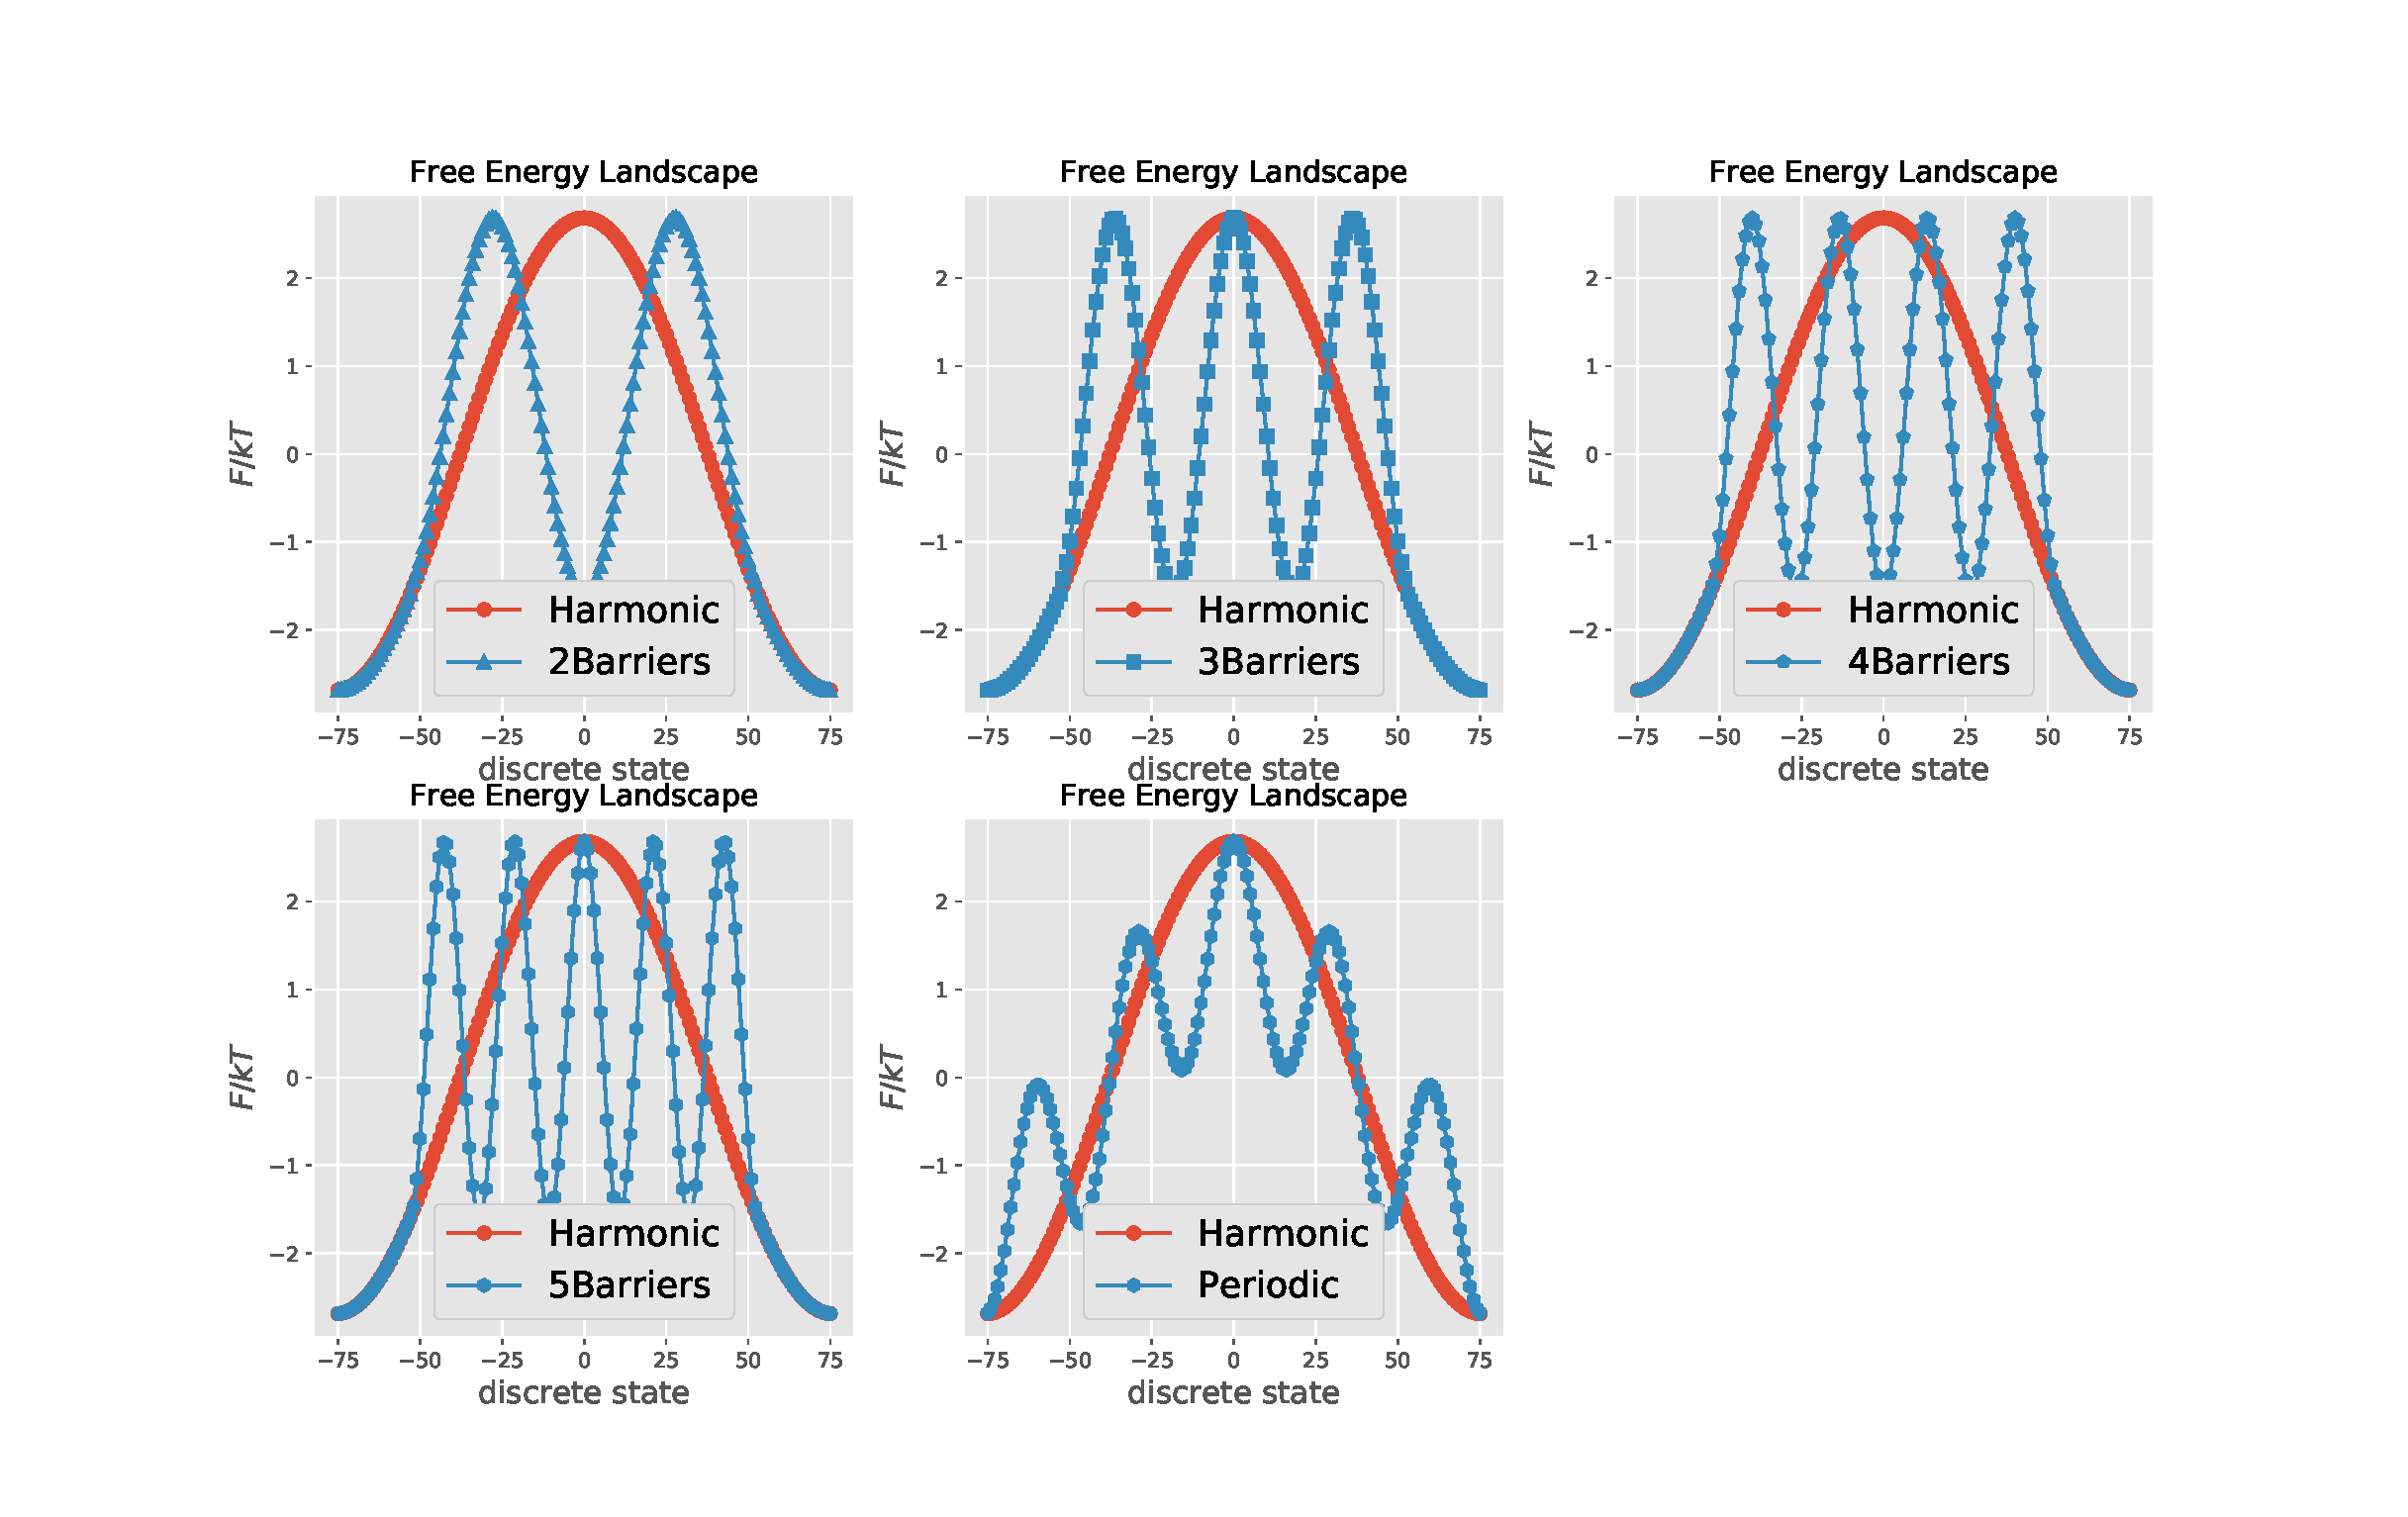
\includegraphics[width=\textwidth]{FELs.eps}}
  \caption{Model free energy landscapes.}
  \label{fig:FEL}
\end{figure}

\subsection{Transition-path transit time distribution}

\paragraph{}Ultilizing Kinetic Monte Carlo simulation for above-mentioned 1-d discrete states models, we sampled 10000
 transition-path trajectories and calculated distribution of transition-path transit times $p(t_{AB})$ for each model landscapes (Figure \ref{fig:tpt_time}).

\begin{figure}[htp]
  \noindent\makebox[\textwidth]{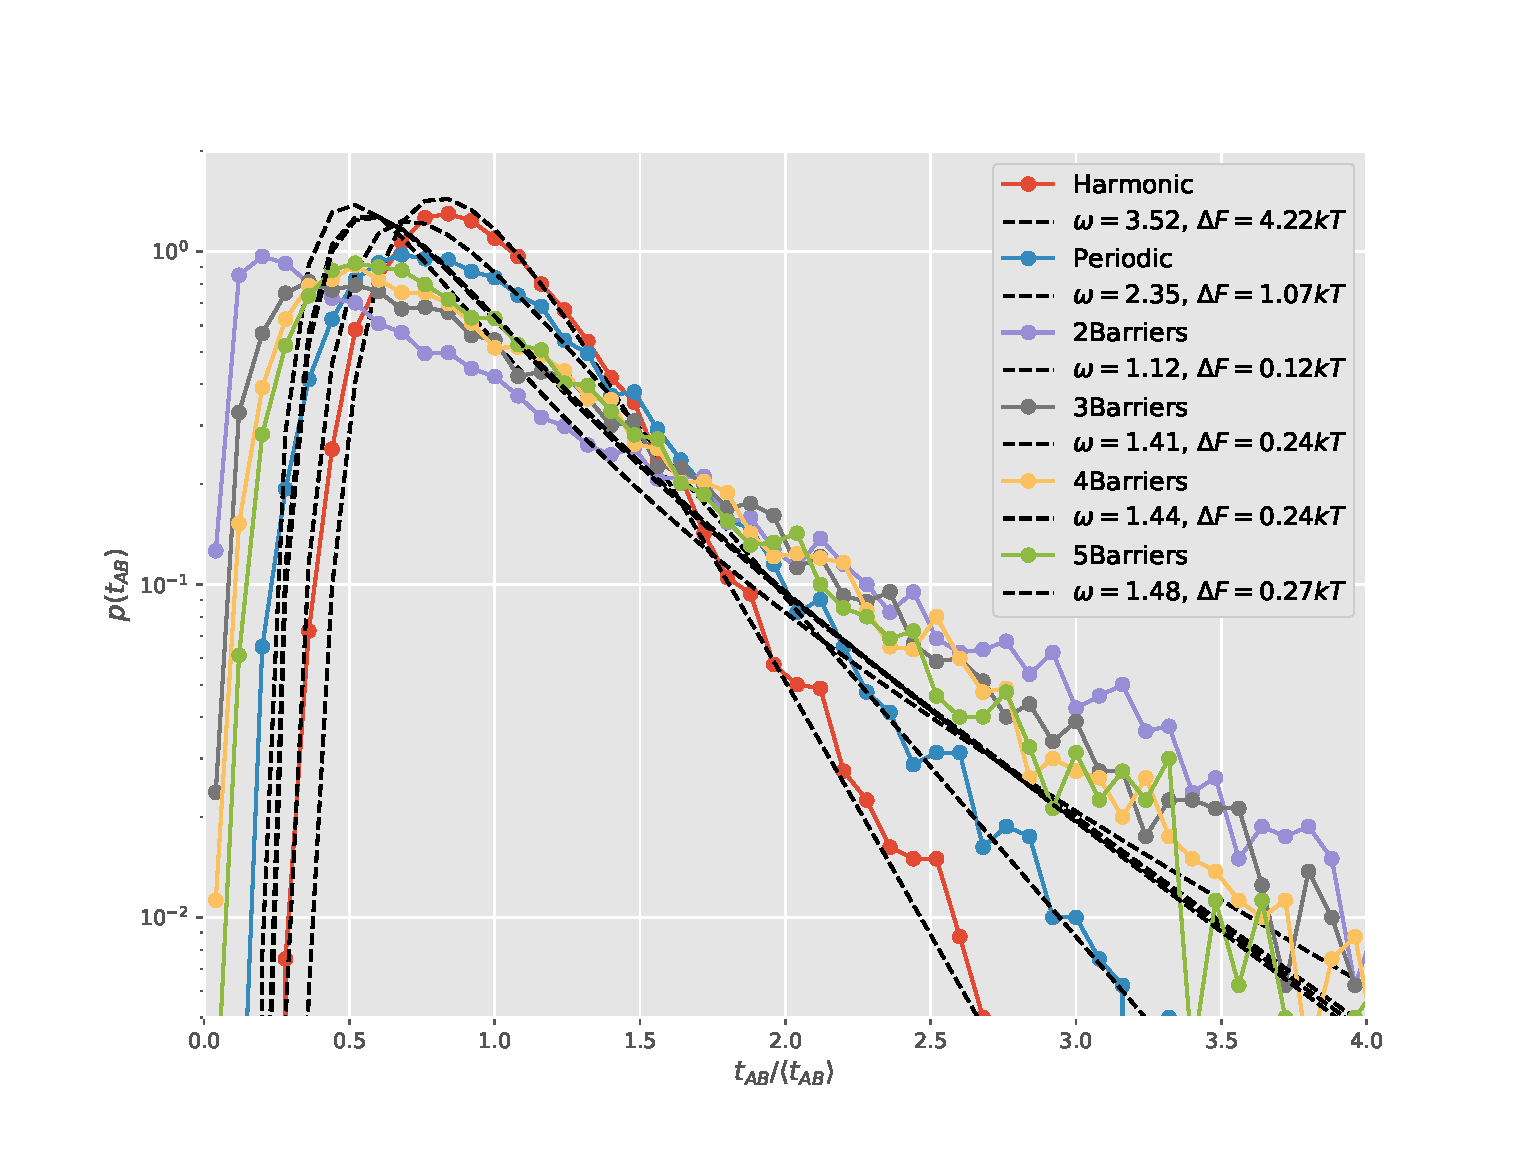
\includegraphics[width=\textwidth]{Transit_Time_distribution_log.eps}}
  \caption{Transition-path transit time distribution.}
  \label{fig:tpt_time}
\end{figure}

\paragraph{}The apparent force constant of the barrier $\omega$ was determined by fitting the decay constant $\omega^{-1}$ of the exponential tail($p(t_{AB}>1.5)$); barrier height $\Delta F$ was
 then determined by fitting theoretial expression of $p(t_{AB})$ to simulated distribution of transit times. We demonstrated that even for the harmonic landscape, deviation from theoretial expression for parabolic barrier crossing is
 non-negligible; for multi-harmonic barriers model, significant deviation from theoretical distribution was observed, resulting in much smaller and relatively unphysical fitting result for barrier height $\Delta F$.

\paragraph{}Interestingly, it appeared that $p(t_{AB})$ of 2Barriers model showed the most significant deviation to the harmonic model; the peak shifted to larger $t_{AB}$ when more intermediate barriers were added.

\subsection{Finite time displacement distribution}

\paragraph{}We also calculated the distribution of finite time displacement as a 1-d collective variable (Figure \ref{fig:dx}). `Fat tail' behavior for multi-barriers models is more significant than the periodic model; when more intermidate barriers is added,
 a second peak emerged near the main gaussian peak, and the distance between main and the second peak is comparable to distance between intermediate barriers.

\begin{figure}[H]
  \noindent\makebox[\textwidth]{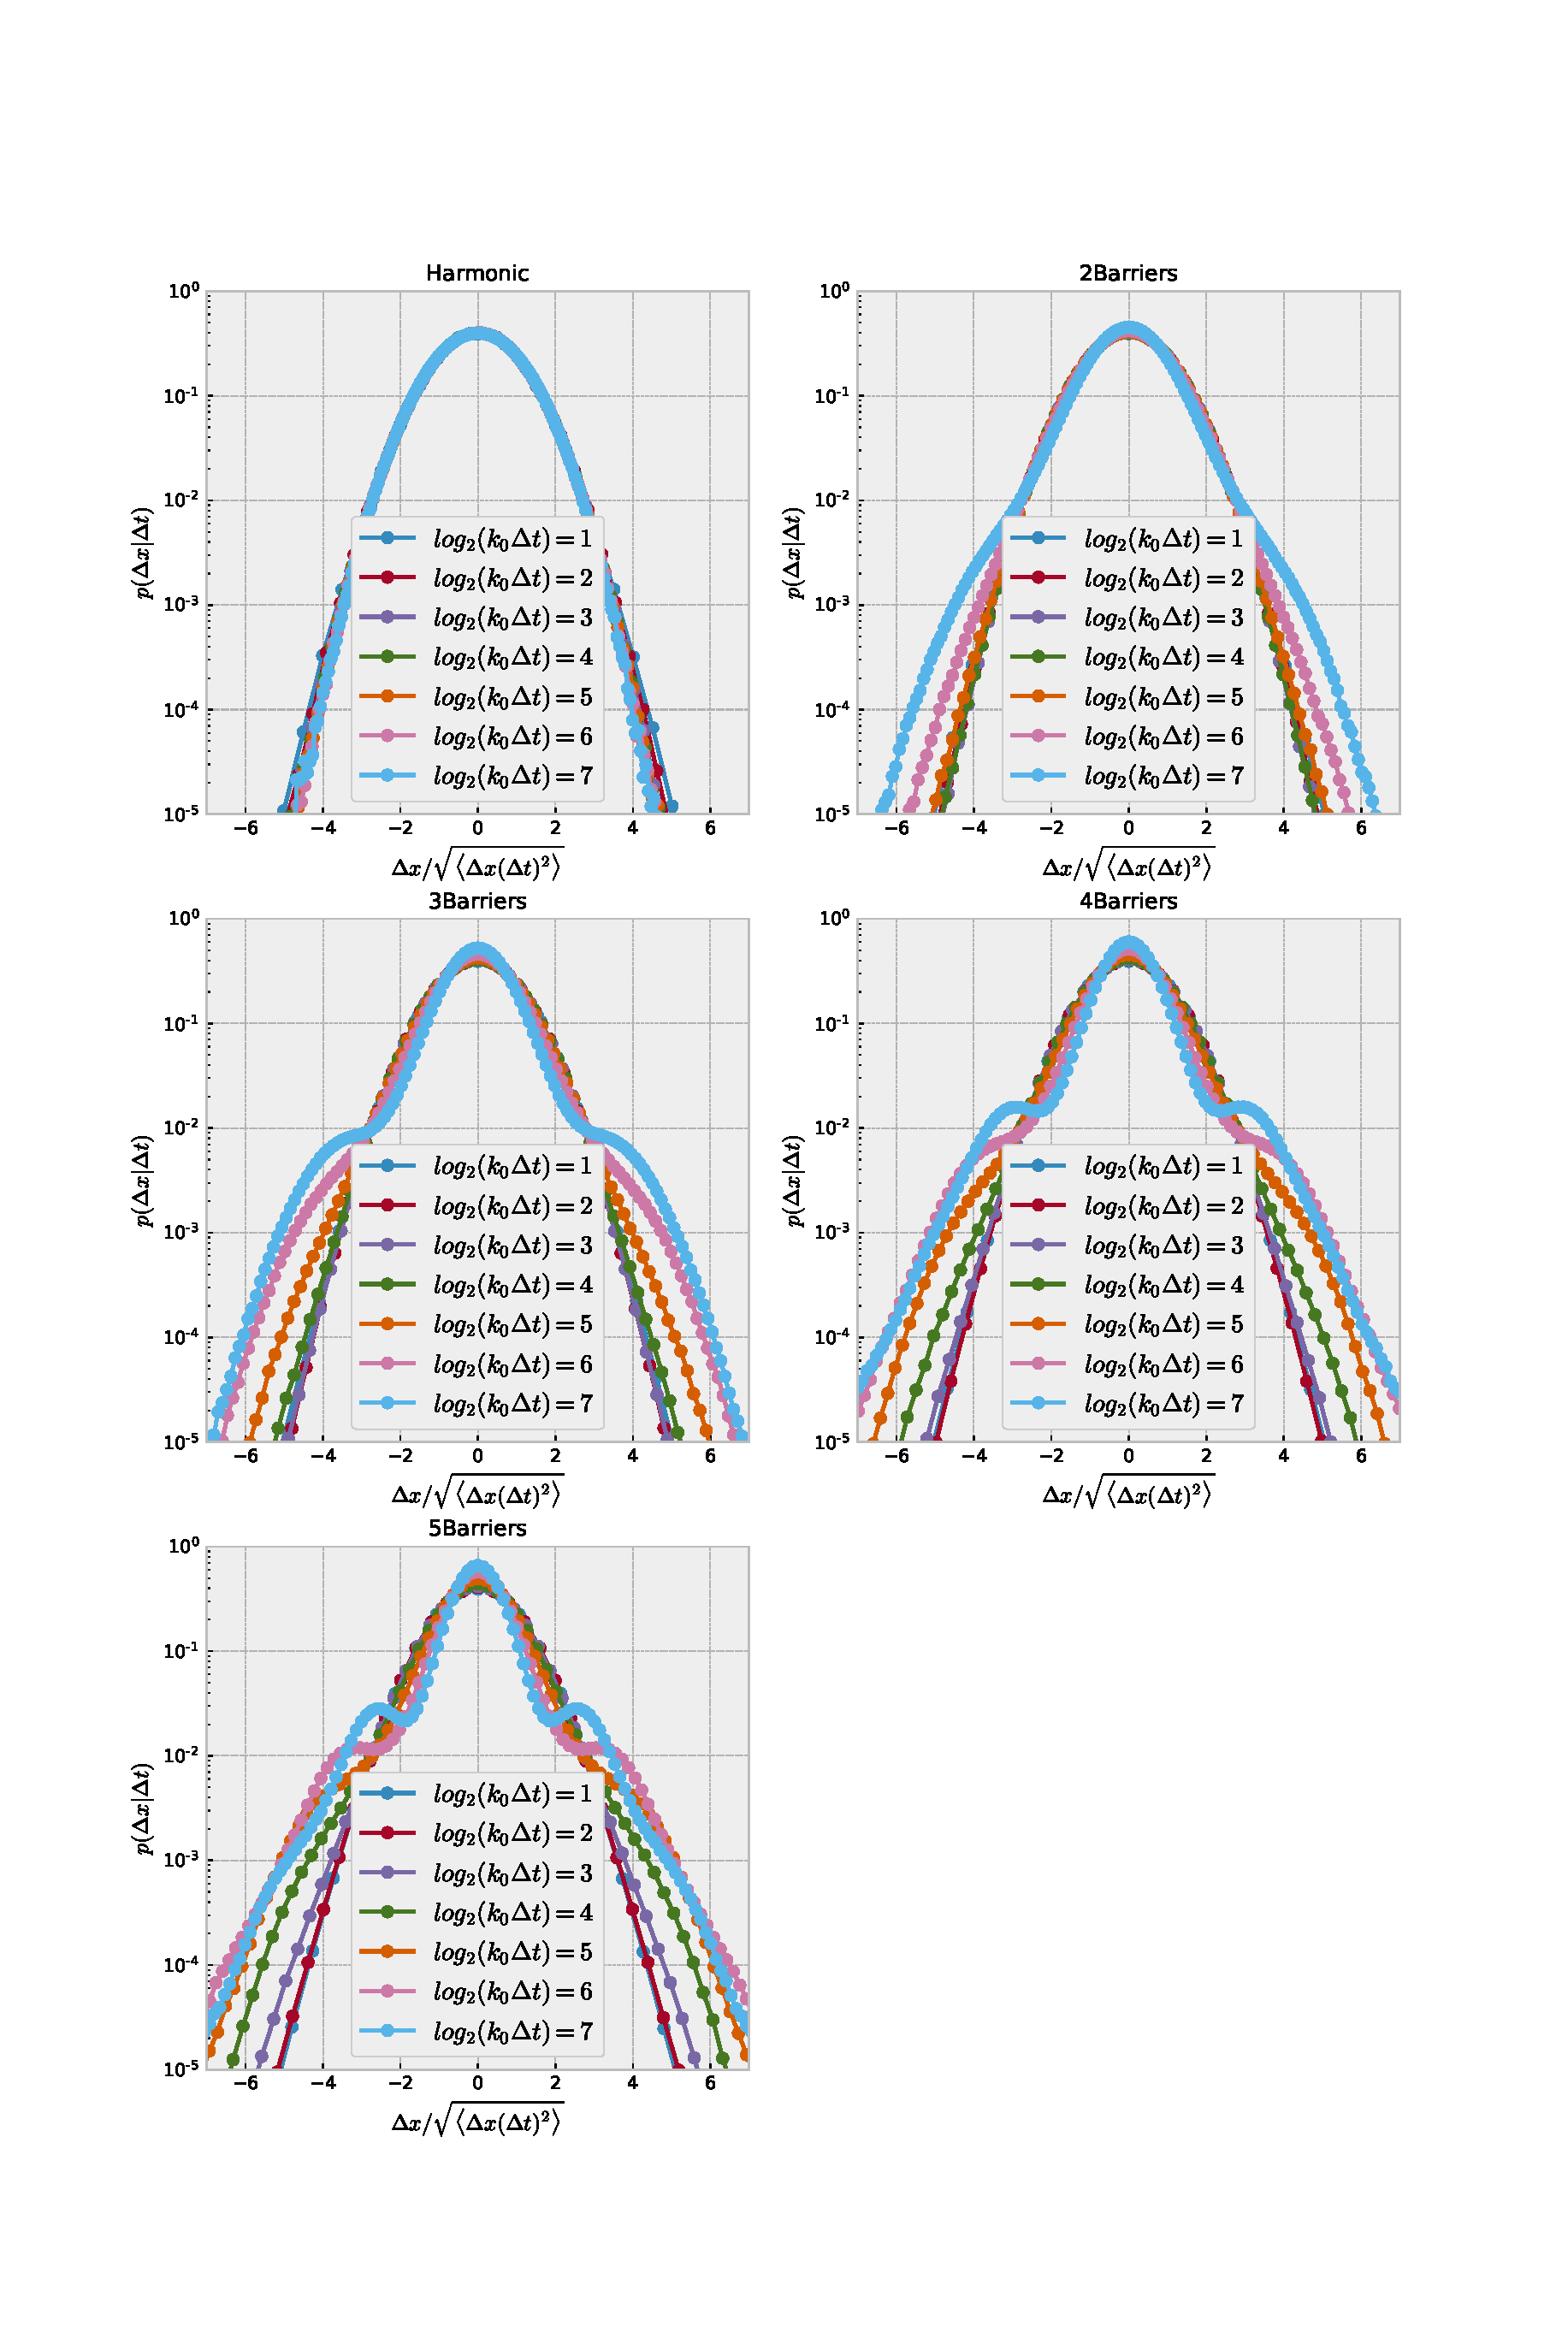
\includegraphics[width=\textwidth]{Finite_time_Displacement.eps}}
  \caption{Distribution of finite-time displacements.}
  \label{fig:dx}
\end{figure}

\subsection{Transition path trajectory crossing probability distribution}

\paragraph{}As a second test, I also calculated the probability density $P(TP|x)$ that an arbitrary trajectory crossing state $x$ is a transition path trajectory(Figure \ref{fig:tpx}) based on distribution of steady state probability and committor distribution;
 for two barriers model, a constant plateau emerged near the barriers region,
 which could be attributed to barrier recrossing due to stabilizing effect of the intermediate free energy well; however when more intermidate energy well was introduced, stepwise falling of $p(TP|x)$ was observed.

 \begin{figure}[htp]
   \noindent\makebox[\textwidth]{\includegraphics[width=\textwidth]{TP_distribution.png}}
   \caption{Probability distribution for transition-path trajectory crossing.}
   \label{fig:tpx}
 \end{figure}
 \begin{figure}[htp]
   \noindent\makebox[\textwidth]{\includegraphics[width=\textwidth]{FELs_2.eps}}
   \caption{Toy free energy landscapes for harmonic model, high frequency model, and flatted harmonic model.}
   \label{fig:FELs_2}
 \end{figure}


\paragraph{}To find a physical explanation for the shapes of $p(TP|x)$ and $p(t_{AB})$, we assume that intermediate free energy wells could be treated as coarse-grained states, and when infinite number of barriers is introduced, the whole free energy landscape could be reduced to asymptotic landscape of discrete CG states,
meaning that time scale of high frequency oscillation and intermidate barrier crossing is well separated. For the cases of finite intermidate free energy wells, it's possible that the `coupling' between oscillation at local free energy minimums and global barrier crossing is
non-negligible, causing large deviation of $p(t_{AB})$ to theoretical distribution.

\begin{figure}[htp]
  \noindent\makebox[\textwidth]{\includegraphics[width=\textwidth]{TP_distribution_cp.png}}
  \caption{Comparision of $p(TP|x)$ for harmonic, flattened harmonic, 2 barriers and high frequency barriers free energy models.}
  \label{fig:tpx_cp}
\end{figure}
\paragraph{}To preliminarily test this assumption, we constructed a model free energy landscape with 50 intermediate barriers('Highfreq'), as well as a 'flatted' harmonic model in which $\Delta F= 1.34 kT$ (Figure \ref{fig:FELs_2}).
I repeated $p(TP|x)$ calulation for these models (Figure \ref{fig:tpx_cp}), and the result showed that the distribution of $p(TP|x)$ of high frequency model strongly resembled the flatted harmonic model near the barrier region,
 indicating well separation of time scale for the high frequency free energy landscape model.

\textbf{That result is probably important for giving explanation to the fact that protein folding transition-path statistics can be described
 by one-dimentional coordinate, but the empirical $\Delta F$ is much lower than real barrier height.}

\section{Future plan}

\paragraph{a.} KMC sampling for transition paths on high frequency model and flattened harmonic model is required to further test the assumption in $2.4$, which can be finished on next week; larger scale simulation is also needed to refine transit time distribution data.
\paragraph{b.} Deciding future proposal for synonymous codon usage project.

%In order to examine when the one-dimensional coordinate projection could be recognized as effective reaction coordinate,
%we then examine the probability distribution of committors for transition path trajectories $p(q|TP)$, for which a single peak of probability $p(q|TP)$ have been ultilized as a indicator for 'good' reaction coordinates.
% Firstly, We found that for harmonic toy model, the shape of $p(q|TP)$ is very sensitive to the definition of source/sink region. For illustration, $p(q|TP)$ for two different selection
%  of source/sink regions was compared: in the first case, only two free energy minimum was indentified as source or sink\textbf{(S1)}; in the second case, only the barrier top was
%  defined as the transition path, while other two region of the free energy landscape was calssified as source/sink\textbf{(S2)}.

%\cite{Jacobs2018,Chaudhury2010,Vanden-Eijnden2010,Metzner,Krivov}

\small
\bibliographystyle{plain}
\bibliography{ref}

\end{document}
